\documentclass[11pt,a4paper]{ctexart}
%以下为所使用的宏包
\usepackage{ulem}%下划线
\usepackage{amsmath,amsfonts,amssymb,amsthm,amsbsy}%数学符号
\usepackage{graphicx}%插入图片
\usepackage{booktabs}%三线表
%\usepackage{indentfirst}%首行缩进
\usepackage{tikz}%作图
\usepackage{appendix}%附录
\usepackage{array}%多行公式/数组
\usepackage{makecell}%表格缩并
\usepackage{siunitx}%SI单位--\SI{number}{unit}
\usepackage{mathrsfs}%数学字体
\usepackage{enumitem}%列表间距
\usepackage{multirow}%列表横向合并单元格
\usepackage[colorlinks,linkcolor=red,anchorcolor=blue,citecolor=green]{hyperref}%超链接引用
\usepackage{float}%图片、表格位置排版
\usepackage{pict2e,keyval,fp,diagbox}%带有斜线的表格
\usepackage{fancyvrb,listings}%设置代码插入环境
\usepackage{minted}%代码环境设置
\usepackage{fontspec}%字体设置
\usepackage{color,xcolor}%颜色设置
\usepackage{titlesec} %自定义标题格式
\usepackage{tabularx}%列表扩展
\usepackage{authblk}%titlepage作者信息
\usepackage{nicematrix}%更好的矩阵标定
\usepackage{fbox}%更多浮动体盒子



%以下是页边距设置
\usepackage[left=0.5in,right=0.5in,top=0.81in,bottom=0.8in]{geometry}

%以下是段行设置
\linespread{1.4}%行距
\setlength{\parskip}{0.1\baselineskip}%段距
\setlength{\parindent}{2em}%缩进


%其他设置
\numberwithin{equation}{section}%公式按照章节编号
\newenvironment{point}{\raggedright$\blacktriangleright$}{}
\newenvironment{algorithm}[1]{\vspace{12pt} \hrule\hrule \vspace{3pt} \noindent\textbf{\color[HTML]{E63F00}Algorithm } \,\textit{#1} \vspace{3pt} \hrule\vspace{6pt}}{\vspace{6pt}\hrule\hrule \vspace{12pt}} % 算法伪代码格式环境


%代码环境\lst设置
\definecolor{CodeBlue}{HTML}{268BD2}
\definecolor{CodeBlue2}{HTML}{0000CD}
\definecolor{CodeGreen}{HTML}{2AA1A2}
\definecolor{CodeRed}{HTML}{CB4B16}
\definecolor{CodeYellow}{HTML}{B58900}
\definecolor{CodePurPle}{HTML}{D33682}
\definecolor{CodeGreen2}{HTML}{859900}
\lstset{
    basicstyle=\tt,%字体设置
    numbers=left, %设置行号位置
    numberstyle=\tiny\color{black}, %设置行号大小
    keywordstyle=\color{black}, %设置关键字颜色
    stringstyle=\color{CodeRed}, %设置字符串颜色
    commentstyle=\color{CodeGreen}, %设置注释颜色
    frame=single, %设置边框格式
    escapeinside=`, %逃逸字符(1左面的键),用于显示中文
    %breaklines, %自动折行
    extendedchars=false, %解决代码跨页时,章节标题,页眉等汉字不显示的问题
    xleftmargin=2em,xrightmargin=2em, aboveskip=1em, %设置边距
    tabsize=4, %设置tab空格数
    showspaces=false, %不显示空格
    emph={TRUE,FALSE,NULL,NAN,NA,<-,},emphstyle=\color{CodeBlue2}, %其他高亮}
}


%节标题格式设置
\titleformat{\section}[block]{\large\bfseries}{Exercise \arabic{section}}{1em}{}[]
\titleformat{\subsection}[block]{}{    \arabic{section}.(\alph{subsection})}{1em}{}[]
% \titleformat{\subsubsection}[block]{\normalsize\bfseries}{    \arabic{subsection}-\alph{subsubsection}}{1em}{}[]
% \titleformat{\paragraph}[block]{\small\bfseries}{[\arabic{paragraph}]}{1em}{}[]


% \titleformat{\sectioncommand}[shape]{format}{title-label}{sep}{before-title}[after-title]



% 中文字号
% 初号42pt, 小初36pt, 一号26pt, 小一24pt, 二号22pt, 小二18pt, 三号16pt, 小三15pt, 四号14pt, 小四12pt, 五号10.5pt, 小五9pt


\begin{document}

\begin{center}\thispagestyle{plain}

{\LARGE\textbf{IEMS 402 Statistical Learning - 2025 Winter}}

{\Large\textbf{HW2}}

Tuorui Peng\footnote{TuoruiPeng2028@u.northwestern.edu}
\end{center}

\thispagestyle{myheadings}\markright{Compiled using \LaTeX}
\pagestyle{myheadings}\markright{Tuorui Peng}




\section{Adaptive to Anisotropic Smoothnes}



We write the $ \hat{m}(x) $ as follows:
\begin{align*}
    \hat{m}(x)=&\dfrac{ \int y\hat{p}(x,y)\,\mathrm{d}y }{ \hat{p}(x) }\\
    =& \dfrac{ \sum_{i=1}^n h^{-2} K(\frac{X_i-x}{h}) \int yK(\frac{Y_i-y}{h})\,\mathrm{d}y }{ \sum_{i=1}^n h^{-1} K(\frac{X_i-x}{h}) }\\
    =& \dfrac{ \sum_{i=1}^n h^{-2} K(\frac{X_i-x}{h}) \int (y-Y_i+Y_i)K(\frac{Y_i-y}{h})\,\mathrm{d}y }{ \sum_{i=1}^n h^{-1} K(\frac{X_i-x}{h}) }\\
    =& \dfrac{ \sum_{i=1}^n  K(\frac{X_i-x}{h}) Y_i }{ \sum_{i=1}^n K(\frac{X_i-x}{h}) }
\end{align*}
which is the same as the kernel regression estimator we defined in class (with window size $ h = 1 $).
\begin{align*}
    \hat{m}_\mathrm{ ker }(x)=   \dfrac{ 1 }{ n }\sum_{i=1}^n W(x)Y_i = \dfrac{ \sum_{i=1}^n K(X_i-x)Y_i }{ \sum_{i=1}^n K(X_i-x) }   
\end{align*}

\section{Implicit Bias of Overparameterized Linear Regression}

\subsection{}

By taking derivative of the empirical risk $ R(w) $ with respect to $ w $, we have:
\begin{align*}
    0=\dfrac{\partial^{}  }{\partial \mathbf{w}^{} }R(w)=& \dfrac{\partial^{}  }{\partial \mathbf{w}^{} }\dfrac{ 1 }{ 2n }\left\Vert \mathbf{X}\mathbf{w}-\mathbf{t} \right\Vert _2^2\\
    =& \dfrac{ 1 }{ n }\big[ \mathbf{X}'(\mathbf{X}\mathbf{w}-\mathbf{t}) \big] \\
     \Rightarrow \mathbf{X}'\mathbf{X}\mathbf{w}=& \mathbf{X}'\mathbf{t}
\end{align*}
which is the expression that the solution $ \hat{w} $ satisfies. In underdetermined case, $ \mathbf{X}'\mathbf{X} $ is not invertible, and the solution is not unique. We may, however, use e.g. the Moore-Penrose pseudoinverse to find a solution such as
\begin{align*}
    \hat{\mathbf{w}}_{\mathrm{ Moore-Penrose } }=(\mathbf{X}'\mathbf{X})^{\dagger}\mathbf{X}'\mathbf{t}
\end{align*}




\subsection{}

With the gradient flow starting from $ \mathbf{w}(0)=0 $, we have the following ODE:
\begin{align*}
    \mathbf{w}(t)=\mathbf{X}'(\mathbf{X}\mathbf{X}')^\dagger\mathbf{t}\big( 1-\exp(-t/n) \big)
\end{align*}

\begin{itemize}[topsep=2pt,itemsep=0pt]
    \item As $ t\to\infty $, we have solution
    \begin{align*}
        \mathbf{w}(t)\to \mathbf{X}'(\mathbf{X}\mathbf{X}')^\dagger\mathbf{t} := \mathbf{w}^*
    \end{align*}
    \item The minimum norm interpolation problem:
    \begin{align*}
        \mathop{ \arg\min }\limits_{\mathbf{w}} \dfrac{ 1 }{ 2 } \left\Vert \mathbf{w} \right\Vert _2^2\quad \text{subject to}\quad \mathbf{X}\mathbf{w}=\mathbf{t}   
    \end{align*}
    its Lagrangian is
    \begin{align*}
        \mathcal{L} =&  \dfrac{ 1 }{ 2 } \left\Vert \mathbf{w} \right\Vert _2^2 + \lambda'(\mathbf{X}\mathbf{w}-\mathbf{t})
    \end{align*}
    with minimizer at
    \begin{align*}
        &\dfrac{\partial^{}  }{\partial \mathbf{w}^{} } \mathcal{L} = \mathbf{w}+ \mathbf{X}'\lambda = 0\\
        \Rightarrow & \mathbf{X}\mathbf{w} = \mathbf{t}= -\mathbf{X}\mathbf{X}'\lambda \\
        \Rightarrow & \lambda = -(\mathbf{X}\mathbf{X}')^\dagger\mathbf{t}\\
        \Rightarrow & \mathbf{w} = \mathbf{X}'(\mathbf{X}\mathbf{X}')^\dagger\mathbf{t}
    \end{align*}
    which is the same as the solution $ \mathbf{w}^* $.

    \item Here I feel that the relation between the traditional predictor and minimum-norm predictor is similar to the relation between maximum-margin predictor and minimum-norm predictor in SVM. In this relation, the original optimize problem has a tough optimization goal (margin $ M $ in SVM, $ \left\Vert Xw-t \right\Vert  $ in regression), by transforming to the minimum-norm predictor, we can throw the difficult part (compute margin for SVM, determine degree of freedom for regression) into the regularization term, and solve the problem with a simpler form.
\end{itemize}


\section{Benefit of Overparameterization}

The result I got is as follows. A similar result as example:
\begin{itemize}[topsep=2pt,itemsep=0pt]
    \item At low degree of freedom (<7): works well, because the regression task is not complex, a relative small degree of freedom is enough to fit the data;
    \item At medium degree of freedom (7-70): significant overfitting and we see some terrible deviation from the true function;
    \item At high degree of freedom (>70): due to the overparameterization, whenever there are some data points at some region, the fitted model would be close to the data points, and thus could be close to the ture model.
\end{itemize}

    


\begin{figure}[H]
    \centering
    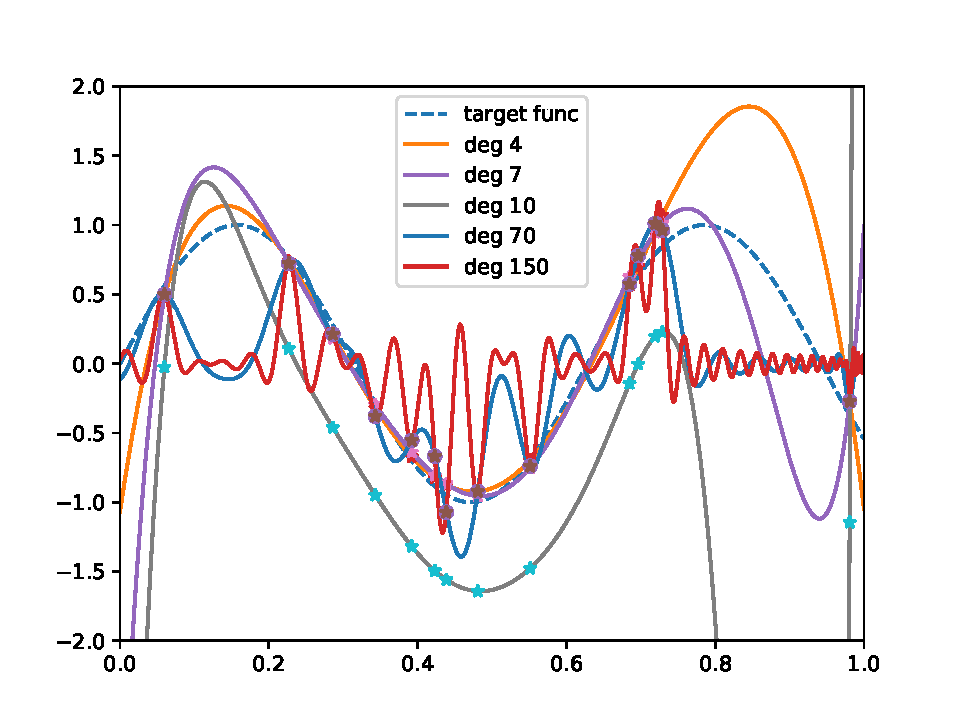
\includegraphics[width=0.8\textwidth]{output.pdf}
    \caption{(Chebyshev) Polynomial Regression: fit v.s. degree of freedom}
\end{figure}

\begin{figure}[H]
    \centering
    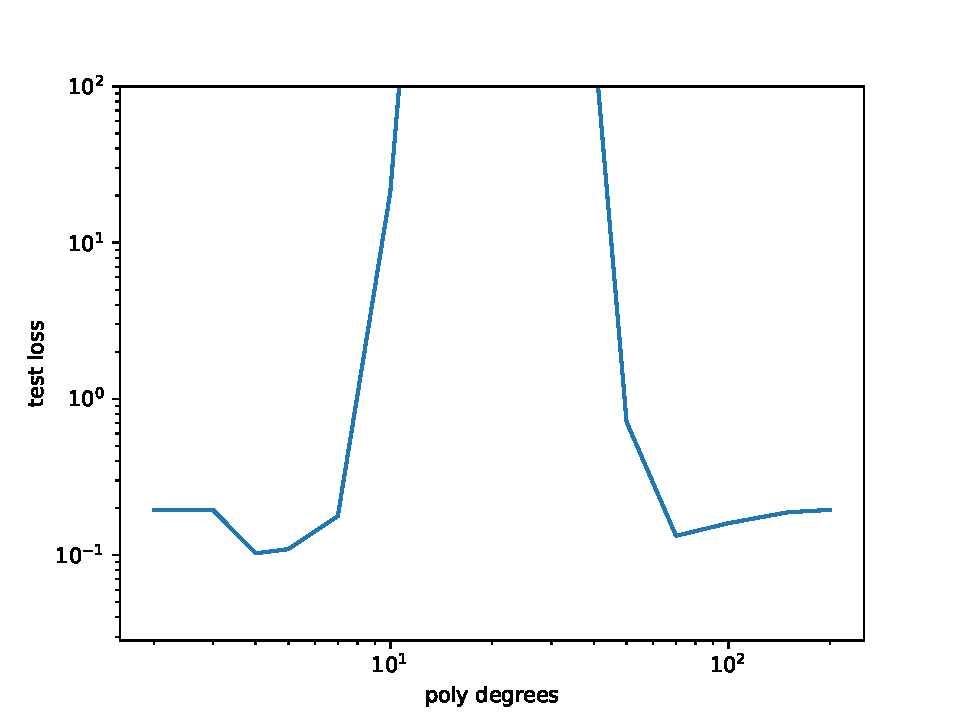
\includegraphics[width=0.8\textwidth]{output_loss.pdf}
    \caption{(Chebyshev) Polynomial Regression: loss v.s. degree of freedom}
\end{figure}









\end{document}